%---------- Inleiding ---------------------------------------------------------

    content...
\section{Introductie} % The \section*{} command stops section numbering
\label{sec:introductie}

Quantum mechanica is een uitdagend onderwerp. Onze intuïties zijn gebaseerd op dagelijkse ervaringen en dus niet op quantum objecten. Quantum objecten lijken in eerste instantie willekeurig en chaotisch maar in realiteit volgen ze “gewoon” een andere set regels. Eenmaal we weten wat deze regels zijn, kunnen we deze gebruiken om nieuwe krachtige technologie te creëren. Quantum computing. 
Quantum computers kunnen problemen oplossen die een klassieke computer nooit zou kunnen. Een voorbeeld van zo’n probleem is het vinden van priem factoren van een enorm groot getal (bv. \(2.55689.10^{29}\)) waarbij de complexiteit een exponentiële groei kent naarmate er cijfers worden toegevoegd.
Machinaal leren is een vertakking van artificiële intelligentie waarbij de focus ligt op het bouwen van applicaties die leren uit data. Aan de hand van deze data gaan de applicaties hun nauwkeurigheid verbeteren zonder expliciet geprogrammeerd te zijn om dit te doen. Data wordt steeds groter, computers worden sterken maar ook algoritmes worden complexer.
Worden algoritmes te complex voor klassieke computers om deze op te lossen? Wanneer bieden quantum computers een meerwaarde voor het oplossen van complexe algoritmes? Kunnen quantum computers klassieke algoritmes oplossen?


%---------- Stand van zaken ---------------------------------------------------

\section{Literatuurstudie}
\label{sec:state-of-the-art}
\subsection{Quantum Computing for Pattern Classification}
'Quantum Computing for Pattern Classification' 
\autocite{Maria Schuld, Ilya Sinayskiy, and Francesco Pertruccione, 2014}. De auteurs introduceren een quantum pattern class algoritme dat gebaseerd is op Trugenberge’s voorstel voor het meten van de Hamming-afstand. Ze bespreken de voordelen van het algoritme met handgeschreven cijfer herkenning van de MNIST-database. 

\subsection{Can Artificial intelligence benefit from quantum computing}
‘Can Artificial intelligence benefit from quantum computing' \autocite{Vincente Moret-Bonillo, 2014}. De auteur opzoek naar relevante karakteristieken van Artificiële Intelligentie en Quantum Computers. Hij benaderd een aantal gevestigde vormen van kunstmatige intelligentie die mogelijk verband houden met werking van biologische hersens. Na het identificeren van gemeenschappelijke kenmerken introduceert de auteur basisconcepten die verband houden met reversable computing en quantum computing die uiteindelijk kunnen helpen om de efficiëntie van huidige vormen van artificiële intelligentie te verbeteren.

% Voor literatuurverwijzingen zijn er twee belangrijke commando's:
% \autocite{KEY} => (Auteur, jaartal) Gebruik dit als de naam van de auteur
%   geen onderdeel is van de zin.
% \textcite{KEY} => Auteur (jaartal)  Gebruik dit als de auteursnaam wel een
%   functie heeft in de zin (bv. ``Uit onderzoek door Doll & Hill (1954) bleek
%   ...'')


%---------- Methodologie ------------------------------------------------------
\section{Methodologie}
\label{sec:methodologie}

In dit onderzoek wordt gezogd naar een complex probleem, een complex algoritme van machinaal leren. Dit complex probleem wordt opgelost aan de hand klassiek computing en aan de hand van quantum computing. Voor het oplossen van het probleem aan de hand klassiek computing wordt gebruik gemaakt van python Scikit-Learn. Voor quantum computing is dit PyTorch en Qiskit.
%---------- Verwachte resultaten ----------------------------------------------
\section{Verwachte resultaten}
\label{sec:verwachte_resultaten}

Naarmate het probleem complexer wordt door het toevoegen van input parameters zal een klassieke computer het probleem veel trager oplossen in vergelijking met een klassieke computer.
\begin{figure}[h]
    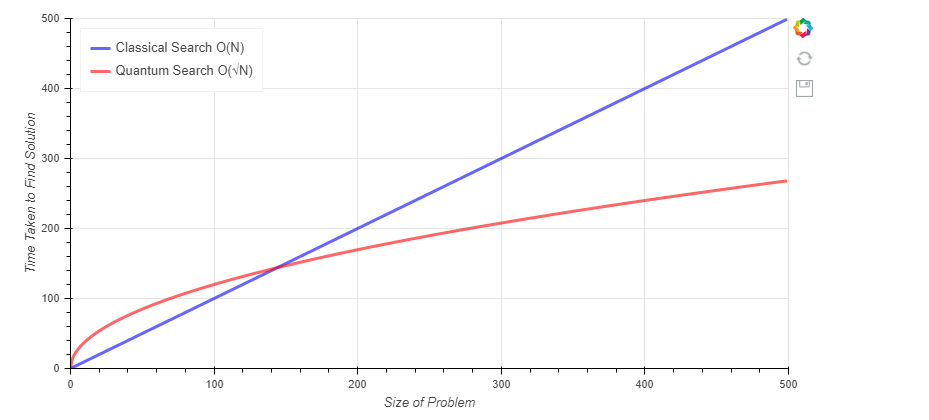
\includegraphics[width=\linewidth]{speed.PNG}
\end{figure}

%---------- Verwachte conclusies ----------------------------------------------
\section{Verwachte conclusies}
\label{sec:verwachte_conclusies}

Er wordt verwacht dat een quantum computer het complex probleem veel sneller zal kunnen oplossen dan een klassieke computer. Alleen gaat de quantum computer geen duidelijke oplossing kunnen geven, of niet hetzelfde probleem kunnen oplossen. Quantum computing technologieën staan nog maar in hun kinderschoen. Om deze reden zou het te vroeg kunnen zijn om te overwegen hoe quantum computers kunnen worden gebruikt op gebied van artificiële intelligentie. 
    

